% TUSP — Branch-and-Price, observability, model correction and LNS
% Build: pdflatex main.tex (twice)
\documentclass[aspectratio=169,9pt]{beamer}

\usepackage[T1]{fontenc}
\usepackage[utf8]{inputenc}
\usepackage[scaled=0.92]{helvet}
\renewcommand{\familydefault}{\sfdefault}
\usepackage{amsmath,amssymb}
\usepackage{booktabs,array,multirow,colortbl}
\usepackage{tikz}
\usetikzlibrary{arrows.meta,positioning,calc,fit,backgrounds,shapes.geometric}
\usepackage{pgfplots}
\pgfplotsset{compat=1.18}
\usepgfplotslibrary{groupplots}
\usepackage{xcolor}

% ------------------------------------------------------------------ colours
\definecolor{navy}{HTML}{0B1F3A}
\definecolor{ink}{HTML}{1E293B}
\definecolor{mute}{HTML}{64748B}
\definecolor{line}{HTML}{CBD5E1}
\definecolor{acc}{HTML}{1D4ED8}
\definecolor{acc2}{HTML}{0891B2}
\definecolor{ok}{HTML}{15803D}
\definecolor{warn}{HTML}{C2410C}
\definecolor{bad}{HTML}{B91C1C}
\definecolor{lav}{HTML}{7C3AED}
\definecolor{soft}{HTML}{F1F5F9}
\definecolor{softacc}{HTML}{E0E7FF}

% ------------------------------------------------------------------ theme
\setbeamertemplate{navigation symbols}{}
\setbeamercolor{normal text}{fg=ink}
\setbeamercolor{structure}{fg=acc}
\setbeamercolor{alerted text}{fg=warn}
\setbeamertemplate{itemize item}{\color{acc}\raisebox{0.15ex}{\scriptsize$\blacksquare$}}
\setbeamertemplate{itemize subitem}{\color{mute}\raisebox{0.2ex}{\tiny$\blacktriangleright$}}
\setlength{\leftmargini}{1.1em}

\newcommand{\tracker}{}
\setbeamertemplate{frametitle}{%
  \vspace{0.22cm}%
  \begin{beamercolorbox}[wd=\paperwidth,leftskip=0.55cm,rightskip=0.55cm]{}%
    {\fontsize{7}{8}\selectfont\color{acc}\bfseries\MakeUppercase{\tracker}}\par\vspace{0.06cm}%
    {\rightskip=0.55cm plus 6em\hyphenpenalty=10000\exhyphenpenalty=10000\fontsize{12.5}{14.5}\selectfont\bfseries\color{navy}\insertframetitle\par}\vspace{0.08cm}%
    {\color{line}\rule{\linewidth}{0.6pt}}%
  \end{beamercolorbox}%
}
\setbeamertemplate{footline}{%
  \begin{beamercolorbox}[wd=\paperwidth,ht=0.55cm,dp=0.2cm,leftskip=0.55cm,rightskip=0.55cm]{}%
    {\fontsize{6.5}{7}\selectfont\color{mute}PORT 2026 · MPRO \quad|\quad Train Unit Shunting: Branch-and-Price, model correction \& LNS\hfill\insertframenumber\,/\,\inserttotalframenumber}%
  \end{beamercolorbox}%
}
\setbeamersize{text margin left=0.55cm,text margin right=0.55cm}

% ------------------------------------------------------------------ helpers
\newcommand{\source}[1]{\par\vfill{\fontsize{6}{7}\selectfont\color{mute}Source: #1}}
\newcommand{\takeaway}[1]{%
  \par\smallskip\noindent\begin{tikzpicture}
    \node[fill=softacc,draw=none,inner sep=3.5pt,text width=\dimexpr\linewidth-11pt\relax,align=left] (t) {\scriptsize\color{navy}\textbf{So what.} #1};
    \fill[acc] (t.north west) rectangle ($(t.south west)+(3pt,0)$);
  \end{tikzpicture}}
\newcommand{\kpi}[3]{% value, label, colour
  \begin{tikzpicture}\node[fill=soft,inner sep=5pt,text width=2.55cm,align=left]{{\Large\bfseries\color{#3}#1}\\[-1pt]{\fontsize{6.5}{7.5}\selectfont\color{mute}#2}};\end{tikzpicture}}
\newcommand{\pill}[2]{\tikz[baseline=(p.base)]\node[fill=#1!12,text=#1!80!black,rounded corners=2pt,inner sep=1.6pt,font=\fontsize{6.5}{7}\selectfont\bfseries](p){#2};}
\newcommand{\shot}[2]{\tikz\node[inner sep=0pt,draw=line,line width=0.4pt]{\includegraphics[#1]{#2}};}
\newcommand{\cbox}[3]{% title, colour, body
  \begin{tikzpicture}\node[draw=#2!45,fill=#2!5,line width=0.5pt,rounded corners=2pt,inner sep=5pt,text width=\dimexpr\linewidth-12pt\relax,align=left]{{\footnotesize\bfseries\color{#2!85!black}#1}\\[2pt]\scriptsize #3};\end{tikzpicture}}
\newcommand{\B}{B\&P}

\begin{document}

% =====================================================================
\begin{frame}[plain]
  \begin{tikzpicture}[remember picture,overlay]
    \fill[navy] (current page.south west) rectangle (current page.north east);
    \fill[acc] ($(current page.south west)+(0,0)$) rectangle ($(current page.south west)+(0.35,9.6)$);
    % stylised time-space network
    \begin{scope}[shift={($(current page.south east)+(-5.4,0.9)$)},opacity=0.5]
      \foreach \x in {0,...,6} \foreach \y in {0,...,4} \fill[white!70!navy] (\x*0.75,\y*0.65) circle (1.5pt);
      \draw[acc2,line width=1.2pt,-{Latex[length=2mm]}] (0,0) -- (0.75,0.65) -- (1.5,0.65) -- (2.25,1.3) -- (3,1.3) -- (3.75,1.95) -- (4.5,1.95);
      \draw[orange!80,line width=1.2pt,-{Latex[length=2mm]}] (0,2.6) -- (0.75,1.95) -- (1.5,1.95) -- (2.25,1.3);
      \draw[red!70,line width=1.6pt] (2.05,1.1) -- (2.45,1.5) (2.05,1.5) -- (2.45,1.1);
    \end{scope}
  \end{tikzpicture}
  \vspace*{1.2cm}
  {\color{acc2}\fontsize{9}{11}\selectfont\bfseries PROOF OF CONCEPT · OPERATIONS RESEARCH}\par\vspace{0.35cm}
  \begin{minipage}{10.5cm}\raggedright\hyphenpenalty=10000{\color{white}\fontsize{20}{24}\selectfont\bfseries Train Unit Shunting: from a black-box solver to an observable, corrected and benchmarked optimisation pipeline\par}\end{minipage}\par\vspace{0.4cm}
  {\color{white!75!navy}\small Branch-and-Price · column generation · a model flaw found by visual inspection · a pricing-based LNS}\par\vfill
  {\color{white!80!navy}\footnotesize BACCAR Bedis \;·\; ESTEVE Erwann \;·\; VERBOIS Maël\\ Projet PORT 2026 — Master Parisien de Recherche Opérationnelle\\[2pt]}
\end{frame}

% =====================================================================
\renewcommand{\tracker}{Executive summary}
\begin{frame}{An observable, audited, physically valid solver, plus a fast primal method}
  \begin{columns}[T,onlytextwidth]
    \column{0.49\textwidth}
    \cbox{1 · Observability}{acc}{Instrumented the \B\ (event trace: CG iterations, tree nodes, bounds, incumbents, root LP) and built a web app that replays any solution on the station map from $t=0$ to $T$ and every solve on its own clock.}\par\smallskip
    \cbox{2 · Correctness audit}{warn}{The app exposed \textbf{8 solver defects}: a non-deterministic graph (out-of-bounds read), B\&B nodes silently dropped, nodes solved under the wrong restrictions, a decreasing global LB, a time limit not enforced inside CG\ldots\ All fixed and regression-tested.}
    \column{0.49\textwidth}
    \cbox{3 · Model correction}{bad}{Watching the animation revealed trains \textbf{crossing head-on on a single track}. The node-only conflict model allows it: \textbf{89 crossings} in the 10 Gurobi solutions. Fixed with exact link resources; the pricing algorithm is unchanged and the reduced costs stay exact (66\,548 columns cross-checked).}\par\smallskip
    \cbox{4 · Large Neighbourhood Search}{ok}{A second method reusing pricing and Lagrangian bounds: greedy insertion \emph{by the pricing oracle}, price-and-dive repair, neighbourhoods pruned by their bound (91\,\% cut on small~1). Feasible solution in ms on every instance; matches \B\ on small~1 in 11\,s.}
  \end{columns}
  \takeaway{The original results (gaps 0–72\,\%) were produced by a model that allows physically impossible plans. Report the corrected model; use \B\ for bounds and LNS for fast, valid plans on large scenarios.}
\end{frame}

% =====================================================================
\renewcommand{\tracker}{Problem}
\begin{frame}{TUSP: route, park and service each train in its window, or refuse it}
  \begin{columns}[T,onlytextwidth]
    \column{0.47\textwidth}
    \textbf{Decisions} for each train $k$ with stay $[a_k,d_k]$ and required services $S_k$:
    \begin{itemize}\setlength\itemsep{1pt}
      \item a path through the station: arrival at an in/out node, shunting moves, services on capable nodes, storage / turning, dwelling, departure;
      \item or \textbf{refusal} (dummy path) at a penalty cost.
    \end{itemize}
    \textbf{Constraints}: each physical node holds at most one train per time step (incl. headway $t_h$); every required service performed once.\par\smallskip
    \textbf{Costs} (integers): shunting $w_s d + c_{shu}$, service $c_s$, storage $w_{dw} t_{turn} + c_{park}$, dwelling $w_{dw} t_s$, refusal $(w_s + w_{dw} + c_{park} + c_{shu})(d_k - a_k) + 2\sum_s c_s$.
    \column{0.5\textwidth}
    \centering
    \scriptsize
    \begin{tabular}{@{}lrrrr@{}}
      \toprule
      Station & nodes & links & trains (sc.\,1–5) & time-space arcs \\
      \midrule
      small   & 24 & 41  & 8 – 24   & 14\,k – 41\,k \\
      medium  & 46 & 129 & 15 – 55  & 36\,k – 101\,k \\
      large   & 74 & 294 & 25 – 105 & 76\,k – 205\,k \\
      variant & 18 & 19  & 10 – 26  & 13\,k – 98\,k \\
      \bottomrule
    \end{tabular}\par\medskip
    \shot{width=\linewidth}{img/station_layout.jpg}\par
    {\fontsize{6}{7}\selectfont\color{mute} small station, automatic schematic layout (in/out $\to$ throat $\to$ 6 two-ended sidings $\to$ services)}
  \end{columns}
  \source{instance CSV files; arc counts from the C++ graph builder ($t_s=5$).}
\end{frame}

% =====================================================================
\renewcommand{\tracker}{Model}
\begin{frame}{A 3-layer time-space network turns each train\textquotesingle s plan into a path}
  \begin{columns}[T,onlytextwidth]
    \column{0.56\textwidth}
    \centering
    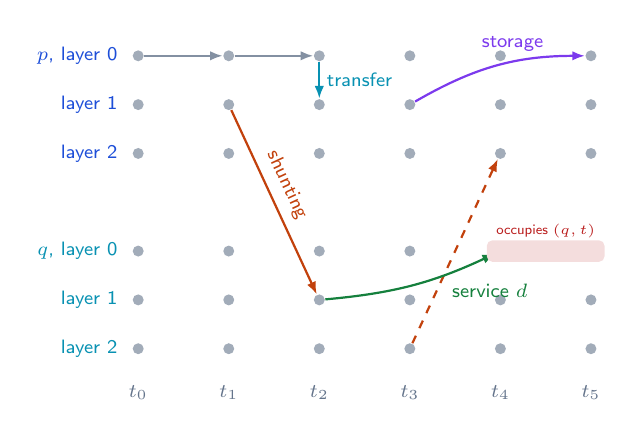
\begin{tikzpicture}[x=1.15cm,y=0.62cm,font=\scriptsize,
        n/.style={circle,fill=mute!60,inner sep=1.4pt},
        a/.style={-{Latex[length=1.6mm]},line width=0.8pt}]
      % two physical nodes p (top) and q (bottom), 3 layers each
      \foreach \t in {0,...,5} {
        \foreach \l/\yy in {0/5,1/4,2/3} \node[n] (p\l\t) at (\t,\yy) {};
        \foreach \l/\yy in {0/1,1/0,2/-1} \node[n] (q\l\t) at (\t,\yy) {};
        \node[mute] at (\t,-1.9) {$t_{\t}$};
      }
      \node[left=4pt,acc] at (p00) {$p$, layer 0};\node[left=4pt,acc] at (p10) {layer 1};\node[left=4pt,acc] at (p20) {layer 2};
      \node[left=4pt,acc2] at (q00) {$q$, layer 0};\node[left=4pt,acc2] at (q10) {layer 1};\node[left=4pt,acc2] at (q20) {layer 2};
      \draw[a,mute!80] (p00) -- (p01); \draw[a,mute!80] (p01) -- (p02);
      \draw[a,warn] (p11) -- node[above,sloped,pos=0.45]{shunting} (q12);
      \draw[a,warn,dashed] (q23) -- (p24);
      \draw[a,ok] (q12) to[bend right=10] node[below right=-1pt,pos=0.7]{service $d$} (q04);
      \draw[a,acc2] (p02) -- node[right=-1pt]{transfer} (p12);
      \draw[a,lav] (p13) to[bend left=15] node[above,pos=0.6]{storage} (p05);
      \fill[bad!15,rounded corners=2pt] ($(q04)+(-0.15,-0.22)$) rectangle ($(q05)+(0.15,0.22)$);
      \node[bad,font=\tiny] at ($(q04)!0.5!(q05)+(0,0.42)$) {occupies $(q,t)$};
    \end{tikzpicture}
    \column{0.42\textwidth}
    \begin{itemize}\setlength\itemsep{2pt}
      \item \textbf{Layer 0} = standing (dwelling, end of service/storage); \textbf{layers 1, 2} = moving in each direction of a link.
      \item Arcs: arrival, shunting (layer $l$, $t\to t+d$), service \& storage (layer $l\to0$), dwelling, state transfer ($0\to l$), departure, \textbf{dummy} (refusal).
      \item Each arc carries its occupation list $\mathrm{occ}(a)\subseteq\mathcal R\times\mathcal T$: the resources it blocks (node $p$ at $t$; headway $t_h$ after a departure).
      \item Train-specific access: storage arcs per train type, service arcs only if $s\in S_k$.
    \end{itemize}
    \scriptsize\color{mute} small sce\,1: 14\,043 arcs, of which 8\,448 storage, 2\,706 shunting, 770 service.
  \end{columns}
  \takeaway{Any feasible plan of one train is a source–sink path; conflicts between trains live only in $\mathrm{occ}(a)$, which is exactly what the master problem couples.}
\end{frame}

% =====================================================================
\renewcommand{\tracker}{Model}
\begin{frame}{Dantzig–Wolfe: one path column per train, unit-capacity coupling rows}
  \begin{columns}[T,onlytextwidth]
    \column{0.52\textwidth}
    \vspace{-2pt}
    \begin{align*}
      \min\ & \textstyle\sum_{k}\sum_{c\in\Omega_k} \gamma_c\,\lambda_c\\
      \text{s.t.}\ & \textstyle\sum_{c\in\Omega_k}\lambda_c \ \ge 1 && (\pi_k)\ \ \forall k\\
      & \textstyle\sum_{c\in\Omega_k} a^{s}_{c}\,\lambda_c \ \ge 1 && (\alpha_{ks})\ \forall k,\,s\in S_k\\
      & \textstyle\sum_k\sum_{c\in\Omega_k} b^{rt}_{c}\,\lambda_c \ \le 1 && (\mu_{rt}\le 0)\ \forall (r,t)\\
      & \lambda_c \in\{0,1\}\quad(\text{LP: } \lambda\ge0)
    \end{align*}
    \scriptsize $\gamma_c$ path cost, $a^s_c=1$ if $c$ performs $s$, $b^{rt}_c=|\{a\in c:(r,t)\in\mathrm{occ}(a)\}|$.
    \column{0.45\textwidth}
    \begin{itemize}\setlength\itemsep{2pt}
      \item $\Omega_k$ is exponential: columns are generated by \textbf{pricing} (next slide).
      \item The \textbf{dummy column} of each train (refusal) is in the RMP from the start $\Rightarrow$ every restricted master is feasible.
      \item Resources $\mathcal R$ = physical nodes (original model) $\cup$ links (corrected model, slide 13).
      \item Branch-and-Price on top: the LP bound is computed by column generation at every node.
    \end{itemize}
  \end{columns}
  \takeaway{The coupling constraints are generic ``(resource, time) $\le 1$'' rows built from $\mathrm{occ}(a)$: adding a new kind of resource does not change the structure of the master or of the pricing.}
\end{frame}

% =====================================================================
\renewcommand{\tracker}{Model · pricing}
\begin{frame}{Pricing is an RCSPP on a DAG and yields a valid bound at every iteration}
  \begin{columns}[T,onlytextwidth]
    \column{0.47\textwidth}
    \textbf{Reduced cost of an arc} for train $k$:
    \[ \bar c_a = c_a(k) - \!\!\sum_{(r,t)\in \mathrm{occ}(a)}\!\!\mu_{rt} \;-\; \alpha_{ks}\,[a \text{ performs } s\in S_k] \]
    Labels $(v, m)$ with $m\in\{0,1\}^{|S_k|}$ = services done; topological sweep over time; sink reached only with $m=\mathbf 1$.
    Cost $O(|A|\,2^{|S_k|})$ per train. Column added if $\bar c(P)-\pi_k<0$.\par\medskip
    \textbf{Lagrangian bound} (valid at each CG iteration):
    \[ LB = z_{RMP} + \textstyle\sum_k \min\big(0,\ \bar c^{*}_k\big) \]
    \scriptsize CG stops when $|z_{RMP}-LB|/LB\le$ gap (per depth tier, tunable in the app).
    \column{0.5\textwidth}
    \begin{tikzpicture}
      \begin{axis}[width=\linewidth,height=4.5cm,font=\scriptsize,
          xlabel={CG iteration (root, small sce\,1)},ylabel={objective},
          ymin=1000,ymax=17000,scaled ticks=false,yticklabel style={/pgf/number format/1000 sep={\,}},legend style={font=\tiny,at={(0.98,0.97)},anchor=north east,draw=none,fill=white,fill opacity=0.8},
          grid=major,grid style={line,opacity=0.5}]
        \addplot[ok,thick,mark=*,mark size=1.1pt] table[x=it,y=rmp]{data/cg_root_s1.csv};
        \addlegendentry{RMP value $z_{RMP}$ (primal)}
        \addplot[acc2,thick,mark=*,mark size=1.1pt] table[x=it,y=lagr]{data/cg_root_s1.csv};
        \addlegendentry{Lagrangian bound}
        \addplot[mute,dashed] coordinates {(0,1959.5) (17,1959.5)};
        \addlegendentry{LP optimum 1959.5}
      \end{axis}
    \end{tikzpicture}
  \end{columns}
  \takeaway{The RMP starts at the all-refused value (16\,040) and meets the Lagrangian bound after 18 iterations: the root LP bound 1959.5 equals the one of the original Gurobi runs, which validates our test set-up.}
  \source{solver trace, small station sce\,1, corrected model (CLP/CBC test solver; identical root bound with Gurobi).}
\end{frame}

% =====================================================================
\renewcommand{\tracker}{Model · Branch-and-Price}
\begin{frame}{Branch-and-Price: two branching rules, two heuristics, every knob exposed}
  \begin{columns}[T,onlytextwidth]
    \column{0.48\textwidth}
    \textbf{Branching} on a fractional train $k$:
    \begin{itemize}\setlength\itemsep{1pt}
      \item \textbf{service split}: choose $(k,s,\tau)$ balancing the fractional flow of service $s$ started before/after $\tau$, divided by the time gap $\Rightarrow$ left: start $\le\tau$, right: start $>\tau$ (forbidden arcs per train);
      \item \textbf{quantum} (fallback): first arc where the fractional paths of $k$ diverge; outgoing arcs split into two flow-balanced sets.
    \end{itemize}
    \textbf{Node selection}: best-bound first or DFS. \textbf{Heuristics} every $N$ nodes: diving (fix the most integral column, re-price) and a MIP on the restricted master.\par\smallskip
    \textbf{CG gap tiers}: root / depth $\le5$ / $\le10$ / deeper.
    \column{0.5\textwidth}
    \centering\shot{height=2.1cm}{img/bp_tree.jpg}\par
    {\fontsize{6}{7}\selectfont\color{mute} app, Search tree tab: node status replayed on the solver clock}\par\smallskip
    \shot{width=\linewidth}{img/bp_cg.jpg}\par
    {\fontsize{6}{7}\selectfont\color{mute} root CG of small sce\,2: 97 iterations, then tailing-off}
  \end{columns}
  \takeaway{The CG on small\,2 shows the classic tailing-off: ~12 columns per iteration until the very end, most time spent re-solving the master.}
\end{frame}

% =====================================================================
\renewcommand{\tracker}{Baseline}
\begin{frame}{Gurobi baseline (1 h): 26–72\,\% gaps, and the master LP takes the time}
  \begin{columns}[T,onlytextwidth]
    \column{0.5\textwidth}
    \begin{tikzpicture}
      \begin{axis}[width=\linewidth,height=4.1cm,font=\scriptsize,
          xlabel={solver time (s)},ylabel={objective},xmin=0,xmax=3650,ymin=5000,ymax=13000,scaled ticks=false,
          yticklabel style={/pgf/number format/1000 sep={\,}},xticklabel style={/pgf/number format/1000 sep={\,}},
          legend style={font=\tiny,at={(0.98,0.6)},anchor=east,draw=none,fill=white,fill opacity=0.85},
          grid=major,grid style={line,opacity=0.5}]
        \addplot[ok,thick,const plot] table[x=t,y=ub]{data/bp_gurobi_s2.csv};
        \addlegendentry{best integer (UB)}
        \addplot[acc2,thick,const plot] table[x=t,y=lb]{data/bp_gurobi_s2.csv};
        \addlegendentry{global LB (old solver)}
        \node[font=\tiny,ok!70!black,anchor=south west] at (axis cs:300,9900) {9\,822};
        \node[font=\tiny,acc2,anchor=south west] at (axis cs:2600,5850) {5\,806};
      \end{axis}
    \end{tikzpicture}\par
    {\fontsize{6}{7}\selectfont\color{mute} small sce\,2 (12 trains), 396 nodes in 1 h, gap 69\,\%}
    \column{0.48\textwidth}
    \centering\scriptsize\renewcommand{\arraystretch}{0.92}
    \begin{tabular}{@{}lrrrrr@{}}
      \toprule
      inst. & trains & gap \% & nodes & time (s) & master \% \\
      \midrule
      S1 & 8  & 0    & 17  & 0.8   & 49 \\
      S2 & 12 & 69.2 & 396 & 3613  & 66 \\
      S3 & 16 & 41.7 & 115 & 3602  & 89 \\
      S4 & 18 & 32.9 & 131 & 3718  & 87 \\
      S5 & 24 & 26.5 & 11  & 3804  & 94 \\
      M1 & 15 & 0    & 13  & 5.7   & -- \\
      M2 & 25 & 51.6 & 31  & 3697  & 94 \\
      M3 & 35 & 72.4 & 6   & \textcolor{bad}{5911} & 96 \\
      M4 & 45 & 30.6 & 6   & 5074  & 96 \\
      \bottomrule
    \end{tabular}\par\smallskip
    \raggedright\scriptsize \textcolor{bad}{M3 ran 64\,\% over its 1\,h limit} (the deadline was not checked inside CG); M1's master time was negative (non-monotonic clock).
  \end{columns}
  \takeaway{The LB barely moves in 1 h and only 6–31 nodes fit in the time on medium instances: the bottleneck is the master LP and the bound, not the search. This motivated (i) a trustworthy LB, (ii) a primal method that does not depend on the tree.}
  \source{\texttt{results/summary\_benchmark.csv} and \texttt{dynamics\_small\_station\_sce\_2.csv} (original solver, Gurobi). LB values of the original solver are not guaranteed (see slide 11).}
\end{frame}

% =====================================================================
\renewcommand{\tracker}{Observability}
\begin{frame}{Observability end to end: event trace, independent decoder, replay app}
  \centering
  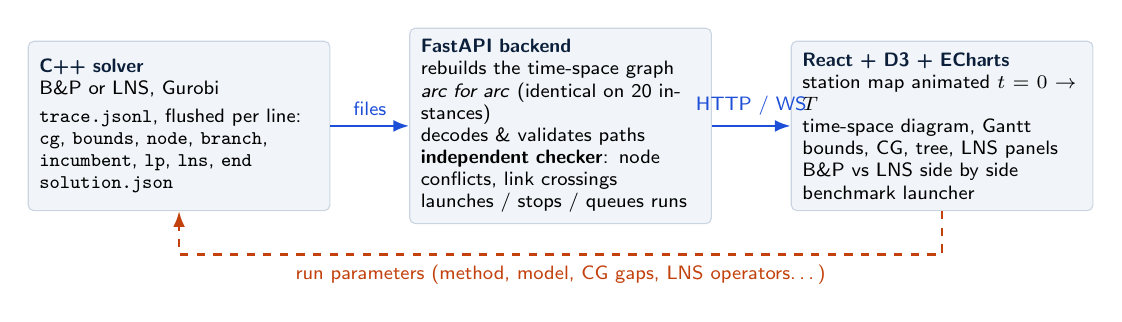
\begin{tikzpicture}[font=\scriptsize,
      box/.style={draw=line,fill=soft,rounded corners=2pt,align=left,inner sep=4pt,text width=3.55cm,minimum height=2.15cm},
      ar/.style={-{Latex[length=2mm]},line width=0.9pt,acc}]
    \node[box] (s) {\textbf{\color{navy}C++ solver}\\ \B\ or LNS, Gurobi\\[2pt] \texttt{trace.jsonl}, flushed per line:\\ \texttt{cg}, \texttt{bounds}, \texttt{node}, \texttt{branch}, \texttt{incumbent}, \texttt{lp}, \texttt{lns}, \texttt{end}\\ \texttt{solution.json}};
    \node[box,right=1.0cm of s] (b) {\textbf{\color{navy}FastAPI backend}\\ rebuilds the time-space graph \emph{arc for arc} (identical on 20 instances)\\ decodes \& validates paths\\ \textbf{independent checker}: node conflicts, link crossings\\ launches / stops / queues runs};
    \node[box,right=1.0cm of b] (f) {\textbf{\color{navy}React + D3 + ECharts}\\ station map animated $t=0\to T$\\ time-space diagram, Gantt\\ bounds, CG, tree, LNS panels\\ \B\ vs LNS side by side\\ benchmark launcher};
    \draw[ar] (s) -- node[above]{files} (b);
    \draw[ar] (b) -- node[above]{HTTP / WS} (f);
    \draw[ar,warn,dashed] (f.south) |- ++(0,-0.55) -| node[pos=0.25,below,warn]{run parameters (method, model, CG gaps, LNS operators\ldots)} (s.south);
  \end{tikzpicture}\par\medskip
  \begin{columns}[T,onlytextwidth]
    \column{0.32\textwidth}\kpi{20 / 20}{instances where the Python graph = the C++ graph (arcs, costs, occupations)}{ok}
    \column{0.32\textwidth}\kpi{89}{head-on crossings found by the checker in the 10 Gurobi solutions}{bad}
    \column{0.32\textwidth}\kpi{live}{trace streamed over WebSocket: curves and tree grow during the solve}{acc}
  \end{columns}
  \takeaway{The decoder never trusts the solver: every displayed plan is re-validated from the instance data, which is what made the bugs and the model flaw visible.}
\end{frame}

% =====================================================================
\renewcommand{\tracker}{Observability · simulation}
\begin{frame}{Replaying a plan makes it readable: here, refusals are 84\,\% of the cost}
  \begin{columns}[T,onlytextwidth]
    \column{0.56\textwidth}
    \shot{width=\linewidth}{img/sim_s4.jpg}\par\smallskip
    \shot{width=\linewidth,trim=0 0 0 120,clip}{img/timespace_s4.jpg}
    \column{0.41\textwidth}
    \scriptsize
    \textbf{small sce\,4 at $t=110$} (Gurobi solution, original model)
    \begin{itemize}\setlength\itemsep{1pt}
      \item tokens move along the links during shunting; rings = service progress; \textsf{P} = storage / turning;
      \item KPIs at $t$: 10 trains in the station, 4 in service, 5/54 services done;
      \item event log and time-space diagram (x = time, y = node) share the same clock; clicking any of them seeks;
      \item cost breakdown of the plan: \textbf{rejection 84\,\%}, service 8\,\%, shunting 5\,\%, dwelling 2\,\%.
    \end{itemize}
  \end{columns}
  \takeaway{18 trains, 8 refused: the objective (36\,815) is dominated by the refusal penalty. Capacity of the service tracks, not routing, is the binding resource; this changes how the LNS chooses neighbourhoods (``refused'' operator).}
\end{frame}

% =====================================================================
\renewcommand{\tracker}{Correctness audit}
\begin{frame}{The audit found 8 solver defects; three invalidate published numbers}
  \scriptsize
  \renewcommand{\arraystretch}{1.18}
  \begin{tabular}{@{}p{3.7cm}p{4.7cm}p{3.1cm}p{2.6cm}@{}}
    \toprule
    \textbf{Defect} & \textbf{How it showed up} & \textbf{Consequence} & \textbf{Fix} \\
    \midrule
    \rowcolor{bad!6} Out-of-bounds read \texttt{services[n]} in the graph builder & arc count 32\,470 vs 32\,174 on small\,4; decoder needed 3 graph variants to read old results & \textbf{graph differs run to run} & loop $s=0..n{-}1$ \\
    \rowcolor{bad!6} Node fetched after a CG prune is skipped & tree in the app had unexplored children marked done & \textbf{``optimal'' not proven} & single \texttt{next\_node()} \\
    \rowcolor{bad!6} Bound-pruned node does not switch state & next node solved with the previous node's forbidden arcs & \textbf{wrong LBs / prunes} & switch before prune \\
    Global LB ignores DFS-pending nodes; child LB overwritten by a weaker Lagrangian bound & Final LB $<$ Root LB (small\,3: 20\,473 $<$ 20\,534) & non-monotone, invalid LB & min over open nodes, $\max$(parent, own) \\
    DFS switch empties the stack & \texttt{-{}-dfs} had no effect & option ignored & transfer pending nodes \\
    Deadline not checked inside CG & 436 s used with a 90 s limit (small\,5); M3: 5\,911 s for 1 h & time limit violated & check in CG, keep best $LB$ \\
    \texttt{high\_resolution\_clock} & negative master time (M1: $-0.85$ s) & wrong profiling & \texttt{steady\_clock} \\
    Benchmark CSV & Final\_LB column contained the UB & misleading table & fixed column \\
    \bottomrule
  \end{tabular}
  \takeaway{The three highlighted defects affect the correctness of bounds or of the search, so the original gaps are not guaranteed. All results after slide 12 come from the fixed solver.}
\end{frame}

% =====================================================================
\renewcommand{\tracker}{Model flaw · discovery}
\begin{frame}{The crossing flaw was spotted in the animation, then measured}
  \begin{columns}[T,onlytextwidth]
    \column{0.33\textwidth}
    {\footnotesize\bfseries\color{navy}1 · Observed in the replay}\par\smallskip
    \shot{width=0.8\linewidth}{img/user_crossing.jpg}\par
    {\scriptsize T3 and T11 on the repair track \texttt{r1-1}–\texttt{r1-2}, moving towards each other in the same step: both ends of one physical track.}\par\smallskip
    {\footnotesize\bfseries\color{navy}2 · Why the model allows it}\par\smallskip
    \tiny
    \begin{tabular}{@{}l@{\hspace{5pt}}c@{\hspace{5pt}}c@{}}
      \toprule
      & step $t$ & step $t{+}5$ \\
      \midrule
      A: $p\to q$ & $(p,t)$ & $(q,t{+}5)$ \\
      B: $q\to p$ & $(q,t)$ & $(p,t{+}5)$ \\
      link $p$–$q$ & \multicolumn{2}{c}{\color{bad}\bfseries never occupied} \\
      \bottomrule
    \end{tabular}\par\smallskip
    {\scriptsize No (node, time) row is shared $\Rightarrow$ the swap is feasible.}\par
    {\scriptsize A shunting arc only occupies its \emph{departure} node at $t_1$ (\texttt{helper\_build\_shunting\_arc}).}
    \column{0.64\textwidth}
    {\footnotesize\bfseries\color{navy}3 · Made systematic: the checker flags every crossing}\par\smallskip
    \centering\shot{height=2.8cm}{img/crossing_alert.jpg}\par
    \raggedright{\fontsize{6}{7}\selectfont\color{mute} Gurobi solution of small\,4 at $t=137$: two crossings in one step (\texttt{p2-2}$\leftrightarrow$\texttt{t3}, \texttt{wt-1}$\leftrightarrow$\texttt{wt-2}).}\par\smallskip
    \begin{columns}[T,onlytextwidth]
      \column{0.55\linewidth}
      \begin{tikzpicture}
        \begin{axis}[ybar stacked,width=\linewidth,height=2.35cm,bar width=5pt,font=\tiny,
            symbolic x coords={S1,S2,S3,S4,S5,M1,M2,M3,M4,L1},xtick=data,ymin=0,
            legend style={font=\tiny,at={(0.5,1.03)},anchor=south,draw=none,fill=none,legend columns=2},
            ylabel={crossings},axis lines*=left,ymajorgrids,grid style={line},ymax=18]
          \addplot[fill=bad,draw=none] table[x=inst,y=inside]{data/crossings.csv};
          \addplot[fill=warn!60,draw=none] table[x=inst,y=throat]{data/crossings.csv};
          \legend{inside one track,between sections}
        \end{axis}
      \end{tikzpicture}
      \column{0.43\linewidth}
      \scriptsize\vspace{4pt}
      \textbf{89 crossings} in 10 solutions:\\
      \textcolor{bad}{\textbf{34}} inside a single track ($X$-1$\leftrightarrow X$-2),\\
      \textcolor{warn}{\textbf{55}} between two sections.\\[2pt]
      The checker reproduces exactly these 89 (unit test).
    \end{columns}
  \end{columns}
  \takeaway{The flaw was invisible in every number (objective, gap, feasibility) and obvious in 2 seconds of animation: visual replay is a verification tool, not a presentation layer.}
\end{frame}

% =====================================================================
\renewcommand{\tracker}{Model flaw · options}
\begin{frame}{Three options: only exact link resources avoid side effects}
  \scriptsize
  \renewcommand{\arraystretch}{1.12}
  \begin{tabular}{@{}p{3.0cm}p{3.6cm}p{3.6cm}p{3.6cm}@{}}
    \toprule
    & \textbf{A · Keep the model} (``each link has one track per direction'') & \textbf{B · Route locking} (a move $p\to q$ also occupies $q$ at $t_1$) & \textbf{C · Link resources} (1 per $\{p,q\}$ and time step, both directions) \\
    \midrule
    New rows & 0 & 0 & $|L|(T/t_s{+}1)$, $\times2.7$–$5$, mostly slack \\
    Nonzeros / column & 0 & $+1$ per move & $+1$ per move ($+18$–$40$\,\%) \\
    Swaps removed & none & all 89 & all 89 \\
    Side effect & 34 swaps happen \emph{inside one track}: physically impossible whatever the links & also forbids \textbf{691} follow-up moves (train entering a section the other just left) $\Rightarrow$ doubles the headway & none: follow-ups and same-direction moves unchanged \\
    Pricing / duals & -- & unchanged (same $\mathrm{occ}$ mechanism) & unchanged (same $\mathrm{occ}$ mechanism) \\
    \midrule
    \textbf{Decision} & \pill{bad}{rejected} not defensible on sidings & \pill{bad}{rejected} changes the model beyond the bug & \pill{ok}{chosen} exact \\
    \bottomrule
  \end{tabular}\par\smallskip
  \footnotesize
  \[ \sum_k\sum_{c\in\Omega_k} b^{\ell\tau}_c\,\lambda_c \le 1 \qquad \forall \ell=\{p,q\}\in L,\ \forall \tau,\qquad b^{\ell\tau}_c = |\{a\in c\cap A_{SH}: \mathrm{link}(a)=\ell,\ t_1(a)\le\tau< t_1(a)+d(a)\}| \]
  \takeaway{Option B looked free (no new rows) but the counts measured on real solutions showed it changes the headway semantics: 8$\times$ more moves forbidden than swaps. Measure side effects before choosing a ``cheap'' fix.}
  \source{counts computed by the decoder on the 10 Gurobi solutions of the original model.}
\end{frame}

% =====================================================================
\renewcommand{\tracker}{Model flaw · correction}
\begin{frame}{Extra occupation entries: pricing unchanged, reduced costs exact}
  \begin{columns}[T,onlytextwidth]
    \column{0.5\textwidth}
    \textbf{Implementation}
    \begin{itemize}\setlength\itemsep{1pt}
      \item resource ids $|P|,\dots,|P|{+}|L|{-}1$ appended to $\mathrm{occ}(a)$ of every shunting arc, \textbf{unordered} pair $\{p,q\}$;
      \item master rows sized by $|\mathcal R|$; arc ids unchanged $\Rightarrow$ old results still decodable;
      \item \texttt{-{}-no-link-conflicts} / app checkbox restores the original model.
    \end{itemize}
    \textbf{Why pricing stays exact.} Master coefficients $b^{rt}_c$ and pricing penalties $\sum_{(r,t)\in\mathrm{occ}(a)}\mu_{rt}$ are built from the \emph{same list}; costs stay additive per arc and the graph stays acyclic, so the DP and the Lagrangian bound are unchanged. A path is on at most one link per step $\Rightarrow$ $b^{\ell\tau}_c\in\{0,1\}$.
    \column{0.47\textwidth}
    \textbf{Verification}\par\smallskip
    \kpi{66\,548}{columns whose pricing reduced cost was recomputed from the master duals: 0 mismatch}{ok}\;
    \kpi{20 / 20}{instances: C++ and Python graphs identical incl. occupations, both models}{ok}\par\smallskip
    \kpi{0}{node conflicts and 0 crossings in every solution of the corrected model}{ok}\;
    \kpi{24 $\to$ 65}{conflict resources on small station (nodes + 41 links)}{acc}\par\smallskip
    \tiny\color{mute} reduced-cost check compiled with \texttt{-DTUSP\_CHECK\_REDUCED\_COSTS}: $\gamma_c-\pi_k-\sum\alpha_{ks}-\sum b^{rt}_c\mu_{rt}$ vs DP value.
  \end{columns}
  \takeaway{The correction is local to the graph builder; correctness of the decomposition is guaranteed by construction and checked at run time.}
\end{frame}

% =====================================================================
\renewcommand{\tracker}{Model flaw · impact}
\begin{frame}{The correction is free at the root and costly in the tree}
  \begin{columns}[T,onlytextwidth]
    \column{0.58\textwidth}
    \centering\scriptsize
    \begin{tabular}{@{}lr|rrl|rrl@{}}
      \toprule
      & & \multicolumn{3}{c|}{original model} & \multicolumn{3}{c}{corrected model}\\
      inst. & root LB & UB & cross. & status & UB & cross. & status \\
      \midrule
      S1 & 1959.5  & 1\,965  & 2 & \textcolor{ok}{optimal 3.7 s} & 1\,974  & 0 & gap 0.46\,\% \\
      S2 & 5438.2  & 12\,259 & 5 & time limit & 12\,504 & 0 & time limit \\
      S3 & 20534.2 & 39\,354 & 7 & time limit & 39\,340 & 0 & time limit \\
      S4 & 27762.2 & 40\,526 & 5 & time limit & 40\,257 & 0 & time limit \\
      \bottomrule
    \end{tabular}\par\smallskip
    \raggedright\scriptsize Root LB \textbf{identical} in both models on every instance (and equal to the Gurobi root LB): crossings appear only in integer solutions.
    \column{0.39\textwidth}
    \cbox{small sce\,1, corrected model, 600 s}{warn}{UB 1\,974, LB 1\,965 (gap 0.46\,\%) after 225 nodes, \textbf{595 s of 600 s spent in primal heuristics} (restricted-master MIP every 5 nodes).\\[2pt] The tuning panel of the app (heuristic frequency, MIP time) is the lever: the tree itself is small.}\par\smallskip
    \cbox{reading}{acc}{The original 1\,965 was only reachable with 2 swaps; the corrected optimum lies in $[1\,965,\ 1\,974]$.}
  \end{columns}
  \takeaway{Report the corrected model. Its LP bound is unchanged, so the weakness of the bound (slide 8) remains the main lever; the extra cost is in branching and heuristics.}
  \source{CLP/CBC test solver, 90 s per run (S1 corrected: 600 s). Absolute times to be re-measured with Gurobi.}
\end{frame}

% =====================================================================
\renewcommand{\tracker}{LNS · design}
\begin{frame}{LNS: destroy a few trains, repair with the pricing, prune with the relaxation}
  \centering
  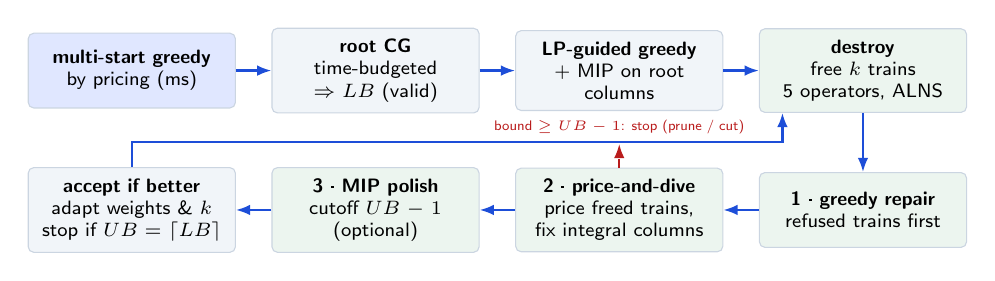
\begin{tikzpicture}[font=\scriptsize,
      st/.style={draw=line,fill=soft,rounded corners=2pt,align=center,inner sep=4pt,minimum height=0.95cm,text width=2.35cm},
      ar/.style={-{Latex[length=1.8mm]},line width=0.8pt,acc}]
    \node[st,fill=softacc] (g) {\textbf{multi-start greedy}\\ by pricing (ms)};
    \node[st,right=0.45cm of g] (r) {\textbf{root CG}\\ time-budgeted\\ $\Rightarrow$ $LB$ (valid)};
    \node[st,right=0.45cm of r] (lg) {\textbf{LP-guided greedy}\\ + MIP on root\\ columns};
    \node[st,right=0.45cm of lg,fill=ok!8] (d) {\textbf{destroy}\\ free $k$ trains\\ 5 operators, ALNS};
    \node[st,below=0.75cm of d,fill=ok!8] (gr) {\textbf{1 · greedy repair}\\ refused trains first};
    \node[st,left=0.45cm of gr,fill=ok!8] (pd) {\textbf{2 · price-and-dive}\\ price freed trains,\\ fix integral columns};
    \node[st,left=0.45cm of pd,fill=ok!8] (mp) {\textbf{3 · MIP polish}\\ cutoff $UB-1$\\ (optional)};
    \node[st,left=0.45cm of mp] (ac) {\textbf{accept if better}\\ adapt weights \& $k$\\ stop if $UB=\lceil LB\rceil$};
    \draw[ar] (g) -- (r); \draw[ar] (r) -- (lg); \draw[ar] (lg) -- (d); \draw[ar] (d) -- (gr); \draw[ar] (gr) -- (pd); \draw[ar] (pd) -- (mp); \draw[ar] (mp) -- (ac);
    \draw[ar] (ac.north) -- ++(0,0.32) -| ($(d.south west)+(0.3,0)$);
    \draw[ar,bad,dashed] (pd.north) -- ++(0,0.3) node[above,font=\tiny,bad,align=center]{bound $\ge UB-1$: stop (prune / cut)};
  \end{tikzpicture}\par\medskip
  \begin{columns}[T,onlytextwidth]
    \column{0.5\textwidth}
    \scriptsize
    \begin{tabular}{@{}ll@{}}
      \toprule
      operator & frees \\
      \midrule
      random & $k$ random trains \\
      time & trains present with a seed train \\
      related & trains sharing nodes and time with a seed \\
      dual & high reduced cost under root duals \\
      refused & refused trains + their competitors \\
      \bottomrule
    \end{tabular}
    \column{0.47\textwidth}
    \scriptsize
    \begin{itemize}\setlength\itemsep{1pt}
      \item weights $w\leftarrow0.8w+0.2\,\sigma$, $\sigma$ = 6 new best / 1 repaired / 0.5 MIP timeout / 0.3 pruned;
      \item $k/n$ grows $\times1.15$ when pruned or stuck, shrinks $\times0.85$ on MIP timeout, restarts after 12 failures at the max;
      \item same trace format as \B\ $\Rightarrow$ same app views + an LNS panel.
    \end{itemize}
  \end{columns}
  \takeaway{Every component reuses the \B\ machinery (RMP, pricing, Lagrangian bound): LNS is a different search over the same decomposition, not a separate model.}
\end{frame}

% =====================================================================
\renewcommand{\tracker}{LNS · pricing \& relaxation}
\begin{frame}{The pricing builds plans; the bound discards 91\,\% of neighbourhoods}
  \begin{columns}[T,onlytextwidth]
    \column{0.45\textwidth}
    \cbox{Greedy insertion = one pricing call per train}{acc}{Insert trains in a given order; for train $k$ set
    $\pi_k = \gamma_{\text{dummy}(k)}$, $\alpha=0$, $\mu_{rt}=-\text{BIG}$ on resources already used.\\
    $\Rightarrow$ the DP returns the cheapest \textbf{conflict-free} path doing all $S_k$, or nothing (refusal cheaper). Feasible plan in $\approx n$ DP sweeps, no MIP.}\par\smallskip
    \cbox{Neighbourhood bound}{ok}{Fixed trains keep one column, already in the RMP $\Rightarrow$ $\bar c^*_k\ge0$:
    \[ LB_N = z_{RMP} + \textstyle\sum_{k\in F}\min(0,\bar c^*_k) \]
    is valid for the restricted problem. Integer costs: if $LB_N \ge UB-1$ the neighbourhood (or the dive step) cannot improve $\Rightarrow$ stop.}
    \column{0.52\textwidth}
    \begin{tikzpicture}
      \begin{axis}[width=\linewidth,height=4.3cm,font=\scriptsize,xlabel={solver time (s)},ylabel={objective},
          xmin=0,xmax=60,ymin=1500,ymax=5600,scaled ticks=false,yticklabel style={/pgf/number format/1000 sep={\,}},
          legend style={font=\tiny,at={(0.98,0.97)},anchor=north east,draw=none,fill=white,fill opacity=0.85},
          grid=major,grid style={line,opacity=0.5}]
        \addplot[only marks,mark=*,mark size=1.1pt,lav] table[x=t,y=lb]{data/lns_s1_pruned.csv}; \addlegendentry{pruned at its bound}
        \addplot[only marks,mark=*,mark size=1.1pt,acc2] table[x=t,y=lb]{data/lns_s1_dive_cut.csv}; \addlegendentry{dive cut by its bound}
        \addplot[only marks,mark=*,mark size=1.1pt,mute] table[x=t,y=lb]{data/lns_s1_no_improvement.csv}; \addlegendentry{repaired, no gain}
        \addplot[ok,thick,const plot] table[x=t,y=ub]{data/lns_s1_ub.csv}; \addlegendentry{best solution (UB)}
        \addplot[mute,dashed] coordinates {(0,1959.5) (60,1959.5)}; \addlegendentry{root LB 1959.5}
      \end{axis}
    \end{tikzpicture}\par
    {\scriptsize small sce\,1, corrected model, 60 s: \textbf{213} neighbourhoods, \textbf{78} pruned + \textbf{116} dive cuts (91\,\%), 0.27 s each; UB 8\,976 (greedy, 0 s) $\to$ 5\,331 (root MIP) $\to$ 3\,650 $\to$ \textbf{1\,974 at 11 s} = \B's best after 600 s.}
  \end{columns}
  \takeaway{The relaxation turns most iterations into a cheap proof that ``no better plan exists here'', so time goes to the neighbourhoods that can still improve. (Trace, CLP/CBC test solver.)}
\end{frame}

% =====================================================================
\renewcommand{\tracker}{LNS · behaviour}
\begin{frame}{The app revealed four failure modes of the first LNS, each fixed by a rule}
  \begin{columns}[T,onlytextwidth]
    \column{0.55\textwidth}
    \scriptsize
    \renewcommand{\arraystretch}{1.2}
    \begin{tabular}{@{}p{2.55cm}p{2.25cm}p{2.5cm}@{}}
      \toprule
      \textbf{Observed} & \textbf{Cause} & \textbf{Rule added} \\
      \midrule
      RMP stuck at 101\,424 for 500 CG iterations (small\,5) & primal degeneracy of restricted masters & stop after 25 iterations without RMP progress (bound kept) \\
      bound $\approx1\,960 \ll UB=3\,650$ yet every dive cut & dive rounded a train's \emph{refusal} column & never round a refusal; fix only columns $\ge0.99$ (conflict-free) \\
      MIP on neighbourhood columns never inserts the refused train & needed columns never priced by the LP & greedy repair inserts refused trains \emph{first} \\
      0 iterations in 90 s (small\,4) & root CG + root MIP used the budget & root CG $\le30\,\%$ of time, root MIP 10 s \\
      \bottomrule
    \end{tabular}
    \column{0.42\textwidth}
    \centering\shot{width=0.86\linewidth}{img/lns_ops.jpg}\par
    {\fontsize{6}{7}\selectfont\color{mute} outcomes per destroy operator (small\,1)}\par\smallskip
    \shot{width=0.86\linewidth}{img/lns_adapt.jpg}\par
    {\fontsize{6}{7}\selectfont\color{mute} ALNS weights and neighbourhood size $k$ over iterations}
  \end{columns}
  \takeaway{With the refusal rule and refused-first insertion, small\,1 went from stuck at 3\,650 to 1\,974 in 11 s. The trace made each failure diagnosable in minutes.}
\end{frame}

% =====================================================================
\renewcommand{\tracker}{Results}
\begin{frame}{\B\ wins when it has time; LNS always has a valid plan in milliseconds}
  \begin{columns}[T,onlytextwidth]
    \column{0.4\textwidth}
    \centering\scriptsize
    \begin{tabular}{@{}lrrrr@{}}
      \toprule
      & \multicolumn{2}{c}{\B} & \multicolumn{2}{c}{LNS} \\
      inst. & UB & 1st sol. & UB & 1st sol. \\
      \midrule
      S1 & \textbf{1\,974} & 3.7 s & \textbf{1\,974} & 0.00 s \\
      S2 & \textbf{12\,504} & 47.9 s & 17\,538 & 0.01 s \\
      S3 & -- & -- & 42\,970 & 0.03 s \\
      S4 & -- & -- & 53\,672 & 0.05 s \\
      S5 & -- & -- & 101\,405 & 0.17 s \\
      \bottomrule
    \end{tabular}\par\smallskip
    \raggedright\scriptsize corrected model, 60 s per run, all plans re-checked: 0 conflicts, 0 crossings. ``--'': no integer solution within the limit.\par\medskip
    \cbox{side by side (small\,2, $t=120$)}{lav}{\B\ refuses T1, T4, T7; LNS refuses T0, T5, T8, T11. Same instance, disjoint refusal sets: the paired schedules show where each method spends service capacity.}
    \column{0.57\textwidth}
    \shot{width=\linewidth}{img/side_maps.jpg}\par\smallskip
    \shot{width=\linewidth}{img/side_diff.jpg}
  \end{columns}
  \takeaway{Complementary roles: \B\ for bounds and quality on small instances, LNS for fast feasible plans where the tree does not produce one. Combining them (LNS incumbent as \B\ cutoff) is the natural next step.}
  \source{app benchmark launcher, CLP/CBC test solver; to be re-run with Gurobi.}
\end{frame}

% =====================================================================
\renewcommand{\tracker}{Validation \& next steps}
\begin{frame}{What is proven, what still needs Gurobi, and the next four steps}
  \begin{columns}[T,onlytextwidth]
    \column{0.48\textwidth}
    \cbox{Proven in this POC}{ok}{\begin{itemize}\setlength\itemsep{0pt}
      \item graph, costs and occupations identical C++ $\leftrightarrow$ decoder (20 instances, both models);
      \item reduced costs exact (66\,548 columns), Lagrangian and neighbourhood bounds valid by construction;
      \item every plan of the corrected model conflict- and crossing-free;
      \item test set-up reproduces the Gurobi root LBs exactly (1959.5, 5438.2, 20534.2, 27762.2, 63822.9).
    \end{itemize}}\par\smallskip
    \cbox{Not yet measured}{warn}{Absolute times and \B\ vs LNS rankings: the CLP/CBC test solver is much slower than Gurobi on the many small re-solves of the LNS and overruns MIP time limits.}
    \column{0.49\textwidth}
    \cbox{Next steps}{acc}{\begin{enumerate}\setlength\itemsep{1pt}
      \item \textbf{Gurobi benchmark}: small + medium $\times$ \{\B, LNS\} $\times$ corrected model, 600 s, 3 seeds, via the app launcher ($\approx$ 1 night).
      \item \textbf{Dual stabilisation} (Wentges smoothing) for the degenerate RMPs that dominate master time.
      \item \textbf{Hybrid}: LNS incumbent as \B\ cutoff from second 1; LNS as a primal heuristic in the tree.
      \item \textbf{Stronger bound}: the LP bound stays far from the UB on scenarios with many refusals (S2: 5\,438 vs 12\,504); study capacity cuts on service tracks.
    \end{enumerate}}
  \end{columns}
  \takeaway{The pipeline is now trustworthy and inspectable; the remaining questions are performance questions, and the tooling to answer them (launcher, traces, side-by-side replay) is in place.}
\end{frame}

\end{document}
